% Appendix E

\chapter{Q-C method and methodology of measurement of parasitic capacities.}\label{app:AppendixE}
\lhead{Appendix E. \emph{Q-C method connection and measurement of parasitic capacities}}

The authors of the method provide a detailed description
in~\cite{App.2, App.3, App.4} of both analog and digital
implementations of the Q-C method.  In both implementations use the
PAR 410 instrument to measure capacitance, instead of which we used
the HP4280a in our case. In addition to the necessary details
concerning the wiring of the method, the authors describe the
methodology for measuring parasitic capacitances or their
elimination. It should be mentioned that the measurement and
elimination of parasitic capacitances can be several procedures can be
followed. In the following, we describe the wiring that we have used
as well as the chosen procedure for measuring parasitic
capacitances. However, for complete mastery of this complex method,
familiarity with the detailed descriptions in~\cite{App.2, App.3,
  App.4} is necessary.

\begin{figure}[h!]\centering
  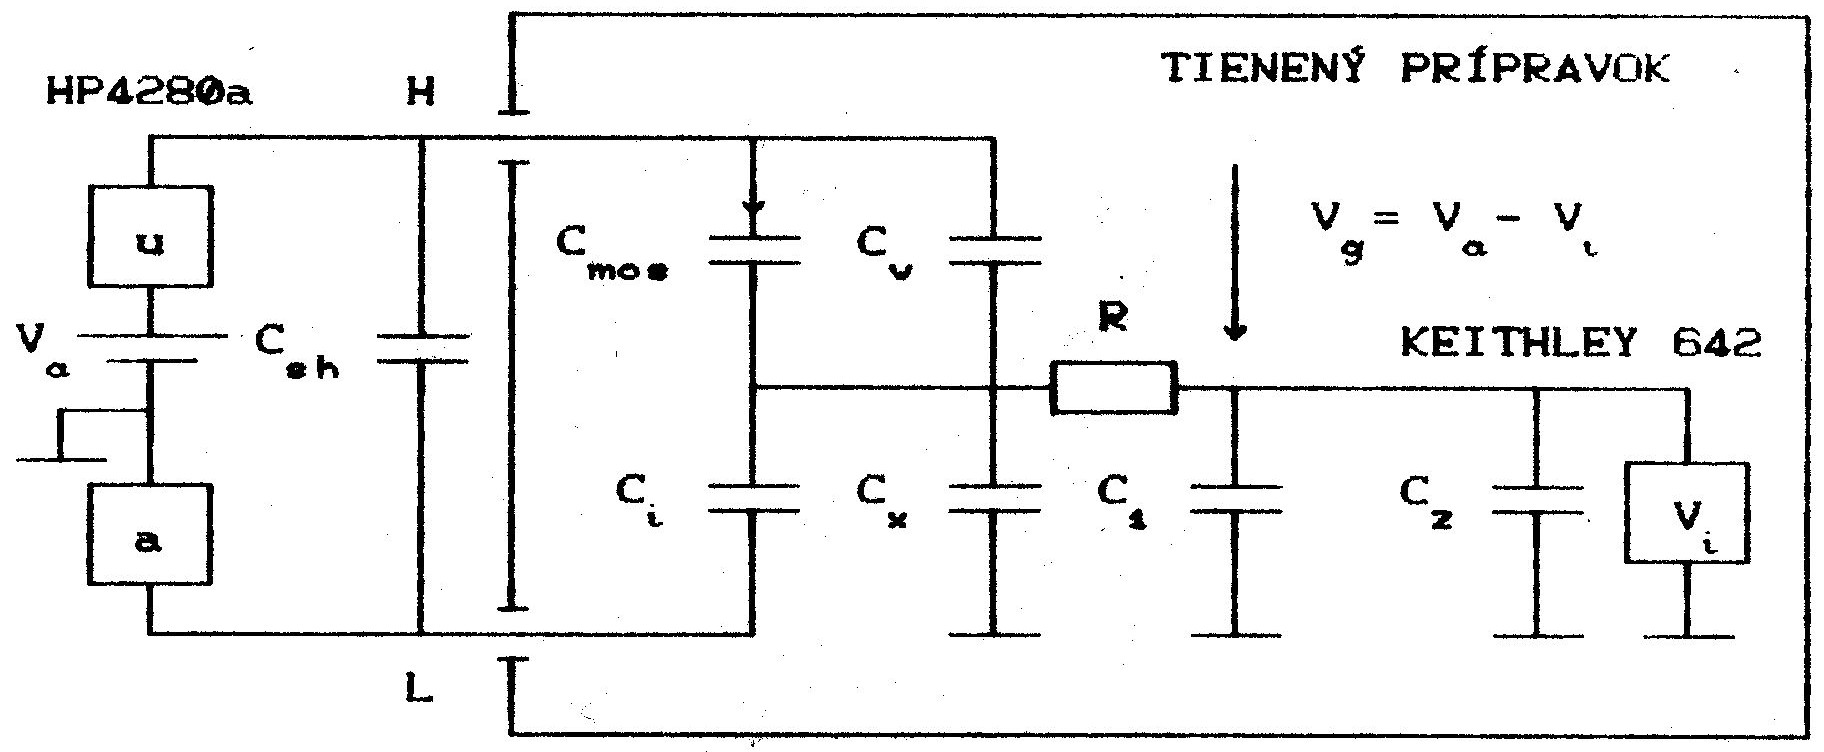
\includegraphics{Figures/fig-app-1.eps}
  \caption[Engagement Q-C method implemented on KME EF
    STU.]{Connection Q-C method implemented at KME EF
    STU.}\label{fig:App.1}
\end{figure}

\par Figure~\ref{fig:App.1} shows the detailed wiring of the workbench
and the measuring instruments of the Q-C method. In the left part of
the figure is shown the measuring instrument HP4280a, which in our
diagram consists of a DC voltage source $V_a$, which is used to
measure structure is brought to the desired state, a source of
high-frequency signal (denoted by u) and an ammeter (denoted by a).
Capacitance $C_{sh}$ represents the parasitic capacitance of the lead
wires, which can be can be eliminated directly by the HP4280a meter
and is therefore will not be considered further. $C_{mos}$ is the
capacitance of the measured structure and $C_i$ represents the
voltage-independent capacitor. Capacitance $C_w$ represents the
parasitic capacitance between the table on which the the structure to
be measured and the raised tip of the probe. $C_x$ indicates the
parasitic capacitance between the common point of connection of the
capacitors (hereafter referred to as common point) and ground. $C_1$
represents the parasitic capacitance of the lead wire to the voltmeter
and $C_2$ indicates the input capacitance of the voltmeter.  These
capacitances $C_1$ and $C_2$ together with the resistance R a low-pass
filter that isolates the voltmeter from the high-frequency signal
generated by the HP4280a. The problem of high frequency measurement is
the fact that the ammeter of the instrument HP4280a does not measure
the component of current flowing from a common point through
capacitors $C_x$, $C_1$ and $C_2$ to ground. This fact should be
should be taken into account when evaluating the high-frequency
measurement. For the final evaluation of the measured data, the
following problems need to be solved:

\begin{itemize}
\item determine the capacitance of $C_i$
\item determination of the parasitic capacitance $C_w$
\item determine the parasitic capacitance $Cx$
\item determine the capacitance of $C_{iLF}  = C_i + C_1 + C_2$
\item correction of the measured high frequency capacitance $C_m$ with respect to
  the current flowing through $C_x + C_1 + C_2$ to ground.
\end{itemize}


\section{Determining the parasitic capacity of $C_w$.}\label{sec:E.1}

A detailed description of the methodology for measuring the parasitic
capacitance $C_w$ is given in the Appendix
2.\ literature~\cite{App.2}. In our experiment, we mentioned
methodology was modified in a way that led to a greater
reproducibility of the results. We describe this procedure.

\begin{enumerate}

\item We connect the MOS structure and at $V_a = 0$ momentarily ground
  the common point to ensure zero external charge on the capacitors.

\item With voltage $V_a$ bring the MOS structure to accumulation and
  read the values $V_a = V_{a0}$ and $V_i = V_{i0}$.

\item Bring the MOS structure into accumulation with a higher voltage
  $V_a$ and read the values $V_a = V_{a1}$ and $V_i = V_{i1}$. From the
  conservation law of charge follows
  \begin{equation}\label{eq:E.1}
  (C_{ox} + C_w)(V_{g1} - V_{g0}) = (C_{iLF} + C_x)(V_{i1} - V_{i0})
  \end{equation}

\item Set $V_a=0$, momentarily ground the common point and pick up the
  probe tip just enough to break contact.

\item Set $V_a \neq 0$ and read $V_a = V_{a2}$ and  $V_i = V_{i2}$.

\item Increase the voltage $V_a$ and subtract the values $V_a =
  V_{a3}$ a $V_i = V_{i3}$. The law of conservation of charge implies
  \begin{equation}\label{eq:E.2}
    C_w(V_{g3} - V_{g2}) = (C_{iLF} + C_x)(V_{i3} - V_{i2})
  \end{equation}

\item By comparing the equations~\ref{eq:E.1} and~\ref{eq:E.2}, we
  obtain the expression to calculate the capacity of $C_w$, which can
  be evaluated, assuming, that we know the capacity of the oxide layer
  of the MOS structure.
  \begin{equation}\label{eq:E.3}
    C_w = C_{ox} \cfrac{1} {\cfrac{\cfrac{V_{g3}-V_{g2}}{V_{g1}-V_{g0}}} {\cfrac{V_{i3}-V_{i2}}{V_{i1}-V_{i0}}} -1}
  \end{equation}

\end{enumerate}

\section{Determining the parasitic capacity of $C_x$.}\label{sec:E.2}

See Appendix 10.\ of the literature~\cite{App.4} for a description of
the direct measurement of the parasitic capacitance of $C_x$. However,
the experimental results show that this measurement is subject to a
large error and its reproducibility is small. Therefore, we have
chosen in our experiment procedure, the principle of which is outlined
in the Appendix 5.\ of the literature~\cite{App.4}. As can be seen in
Appendix~\ref{sec:E.4}, the high-frequency capacitance of the MOS
$C_{mos}$ structure is a function of of the parasitic capacitance
$C_x$ that we wish to determine. In accumulation, the $C_{mos} =
C_{ox}$, which can be achieved by a suitable variation of of $C_x$. In
our evaluation of the data measured by the Q-C method, we variation of
$C_x$, we used the interval division method.

\section{Capacity determination $C_{iLF}$.}\label{sec:E.3}

In Appendix 10.\ of the literature~\cite{App.4} is a description of
the direct measurement of the parasitic capacitance
$C_{iLF}$. However, similar to the measurement of $C_x$, the
experimental results show that this measurement is loaded by a large
error. Therefore, we have chosen a procedure based on the condition,
that the low and high frequency capacitances of the MOS structure must
have the same value in accumulation. The determination of $C_{iLF}$ is
then based on the following relation

\begin{equation}\label{eq:E.4}
  \frac{\delta}{\delta C_{iLF}} \sum\limits_{j} {\Big[C_{mos}^{LF}(j) - C_{mos}^{HF}(j)\Big]}^2 = 0
\end{equation}

, where the above summation is performed for points measured in
accumulation. A description of the derivation of the relation for the
calculation of $C_{iLF}$ is given in the Appendix 4.\ of the
literature~\cite{App.4} and here we only give its final form.

\begin{equation}\label{eq:E.5}
  C_{iLF} = \frac{\sum\limits_{j}{\Bigg[C_{mos}^{HF}(j)+C_{w}\Bigg]}{\Bigg[\cfrac{dV_i}{dV_g}\Bigg]}_j}{\sum\limits_{j}{\Bigg[\cfrac{dV_i}{dV_g}\Bigg]}_j}
\end{equation}

It should be noted that the above procedure has the advantage that its
use guarantees the coincidence of low and high frequency capacitance
dependence of the MOS structure in the accumulation, which constitutes
a good basis for calculation of the interface traps from the two
capacitance dependencies mentioned above.

\section{High frequency capacitance correction $C_m$.}\label{sec:E.4}

In Appendix 1.\ of the literature~\cite{App.2} an analysis of the Q-C
method from a high-frequency measurement perspective. Here we give its
main idea.

\begin{figure}[h!]\centering
  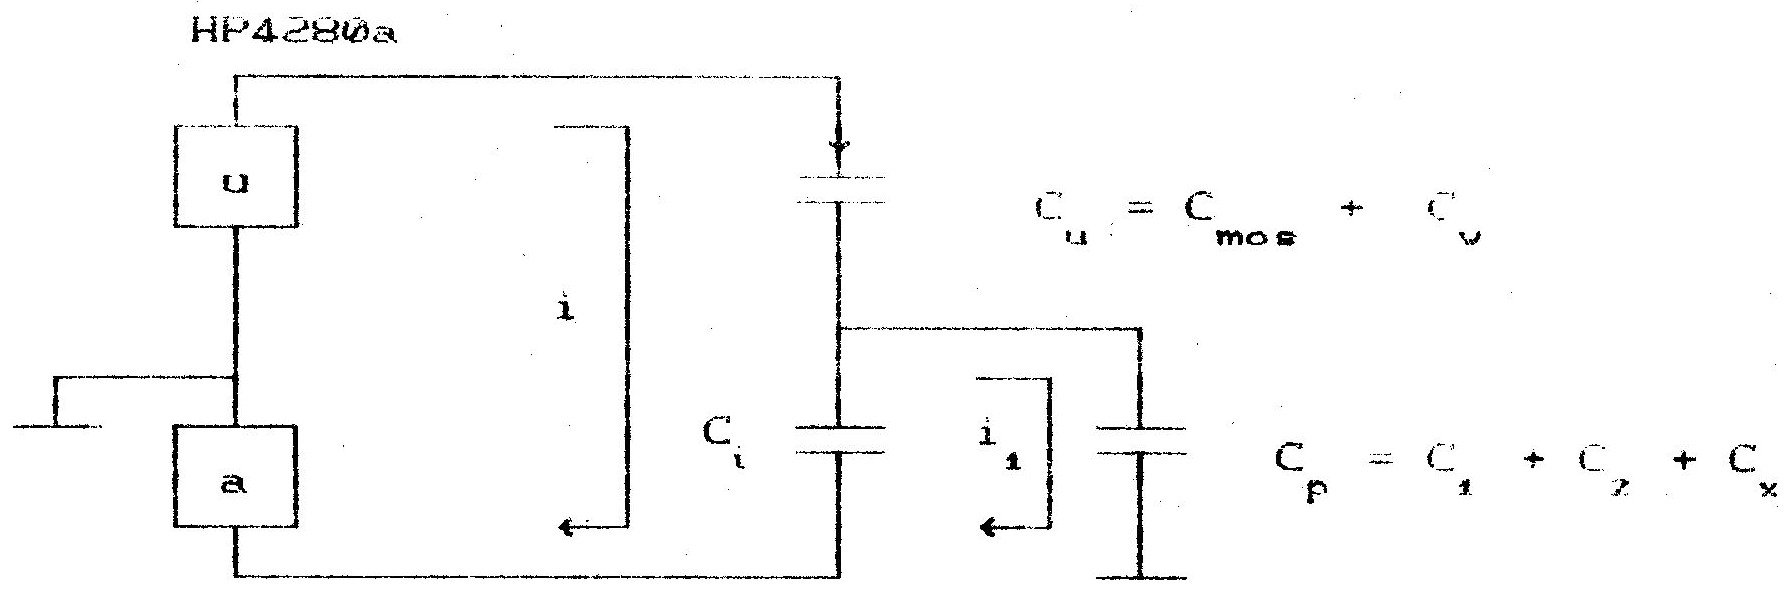
\includegraphics{Figures/fig-app-2.eps}
  \caption[Equivalent wiring of the Q-C method for high-frequency
    measurements]{Equivalent wiring of the Q-C method for
    high-frequency measurement.}\label{fig:App.2}
\end{figure}

As can be seen from the figure~\ref{fig:App.2} ammeter of the HP4280a
instrument does not measure the current $i_1$ flowing through the
capacitor $C_p$. The capacitance $C_m$, which we measure with this
instrument can be expressed by the relation

\begin{equation}\label{eq:E.6}
  C_m = \frac{C_{u} C_{iHF}} {C_{iHF}+C_{u}+C_{p}}
\end{equation}

Chapter~\ref{sec:3.3} gives the relations for calculating of the
frequency capacity of the MOS\@ structure.  In order for the results
obtained from relations~\ref{eq:3.3} are not affected by the above
fact, it is necessary to to make the following corrections (according
to Appendix 1.\ of the literature~\cite{App.4})

\begin{equation}\label{eq:E.7}
  C_{iHF}=C_{iHF}k, \qquad G_{m}=G_{m}k, \qquad C_{m}=C_{m}k
\end{equation}

, where

\begin{equation}\label{eq:E.8}
  k = 1 + \frac{C_x}{C_{iHF}}
\end{equation}
